\documentclass[heading.tex]{subfiles} 
\begin{document}

% \tableofcontents

\section{Introduction}
\subsection{Motivation}
This research was initiated as risk reduction for the NASA
Gondola for High Altitude Planetary Science (GHAPS) mission.
High altitude balloon missions carrying expensive science payloads
across harsh, difficult-to-access locations could greatly benefit from
improved descent and landing systems with the ability to mitigate landing
loads and improve general recoverability.

As a first step, the Rocket University development program developed a series
of payloads of increasing capability to monitor and evaluate various recovery
systems. Comprised mainly of consumer-of-the-shelf (COTS) electronics and
open-source software, this paper offers a few turn-key solutions for highly
cost-constrained science missions. Rather than re-inventing the wheel, these
solutions leverage open-source microcontroller platforms with large ecosystems
that offer both flexibility and simplicity.


\subsection{Balloon Sub-System Basics}

A vast multitude of HAB related resources exist online, therefore many of the
ancillirary subsystems are only breifly outlined here. With many amatuer missions
focused on videography, this work addresses data aquisition and power management;
two disciplines that scale to a wide range of balloon mission.

\subsubsection{Power and Thermal}

Payloads endure extremely cold temperatures, making the most common battery
types undesirable. As temperature decreases, voltage and overall battery
capacity also decreases, often dropping off extremely fast after reaching a specific
temperature threshold. With ambient temperatures reaching down to -75\degree C,
passive inuslation or active heating can greatly improve battery capacity.
Many balloon applications with active heating and radio transmitters also draw
current on the order of amps. Much like cold temperatures, high power draw can
also disproportionately reduce battery life. 

Lithium Sulfer Dioxide (LiSO2) non-rechargeable batteries have been found to 
satisfy all of the typical HAB requirements. They can sustain relatively high
current draw, are resistant down to -40\degree C and their high energy density
is desirable for lighter-than-air applications.
This particular battery chemistry is rated for many space and
medical applications, and are the primary battery type flown by the Columbia
Scientific Balloon Facility.

Using passive thermal insulation alone can capture enough waste heat from the
battery bank to maintain -40\degree C, and on small payloads, chemical heat
from hand-warmers are a popular and extremely simple supplemental heat source.
Waste heat from transmitters and other on-boad electronics can also be used to
keep the payload warm. Given the extremely rarified air at high altitudes,
heat is primarily transferred by direct thermal conduction and radiation.
The lack of convection can be a double-edged sword, helping electronics retain
heat in some cases, but also making it difficult to release unwanted heat
without heat sinks or radiators.

Small scale missions are often airborne on the order of six hours,
requiring multiple batteries connected in both series and parallel.
When building battery banks it's important to consider variations between
battery cells, which become exacerbated by high loads and low temperatures.
Without sophisticated circuitry, it is generally not advisable to connect
batteries into more than two parallel strings. Power across each string is more
likely to become increasingly unbalanced, after a single string starts to degrade.
This creates a positive feedback loop, which can ultimately lead to a dangerous
thermal run-away. With D-cell sized batteries being the limit for most consumer
batteries, this puts a natural limit on the Amp-hour capacity of amatuer flights.


\subsubsection{Telemetry}

The ability to recieve live wirelessly transmitted data from a payload is
essential for the recoverability of any balloon launch. FindMeSpot is the easiest
COTS tracking device, requiring no configuration or operator licenses.
Communication via cell phone devices also offers slightly more flexibility,
but additional configuration and complexity.
Both of these methods are limited to 40,000ft altitude celings.
To maintain constant communication up to 100,000+ feet requires higher powered radios.
The most accessible amatuer radios require an operator with an amatuer HAM license.
These licenses require taking an exam (technical difficulty on par with a
driving exam) from a local amatuer radio chapter. Many free online resources and study
guides provide an easy way to master the finite pool of possible written quiz
questions in a few weeks time. After passing the written test, the basic
technician license is granted by the FCC within a few weeks. Additional licenses
can be obtained by taking increasingly difficult written exams, allowing the
operation of higher powered radios over a larger range of frequencies.

The most popular balloon radio protocol, Automatic Packet Reporting System (APRS)
provides a very succinct transmission including the balloons GPS lat, lon, heading,
and operator call-sign. By commiting to this protocol, the operator is able to
leverage a large amount of pre-existing HAM radio infrastrucutre. Rather than
relying exclusively on personal ground station equipment, many other amatuer
stations are constantly listening for the APRS frequency and protocol. If the
signal reaches any of these stations, the signal will be repeated and re-broadcasted
to neighboring stations. Eventually the signal will reach an internet ``gateway''
where it is published to various web applications and databases.
This allows an APRS operator to simply broadcast signals,
without the direct need for any reciever equipment.
As long as the signal reaches neighboring HAM stations, the call-sign and information
will be available in real-time from any internet connected device.
For more direct reception and faster feedback,
many affordable handheld recievers are available that can
be tuned to filter out all incoming signals except APRS messages from specfic
call-signs.

If the payload requires more advanced telemetry, leveraging other frequencies
and protocols may be more suitable. If a constant transmission
(possibly bi-directional) communication link or higher bandwidth is needed,
amatuer remote control UAV radio components may be a better option.
With balloon operations requiring extremely long-distance communication,
the most ideal frequencies reside in the UHF range.
As a general rule, transmission bandwith increases and range decreases with
increasing frequency. 900Mhz is ideal for
basic telemetry in the 100-200 kbps range up to 40 miles away. Radio modems
include the RFD900, and Xtend900. These specific models are identified for their
drop-in compatibility with existing hobby level UAV ecosystems that are outlined
in subsequent sections. They are only export controlled, require only
a basic technician's license, and require a minimal amount of radio and 
programming experience.

\subsubsection{Balloon and Parachute}

[Jeremiah Section]
Include images, and balloon providers,where to purchase, estimated helium cost,

For small scale balloon missions Kaymont meteorological balloons are our preferred choice.
These balloons are selected due to Kaymont's history of providing high-altitude
weather balloons to the amateur ballooning community.
The balloons are available in a variety of sizes,
selected based on the required mass to be lifted and the final float altitude.
The smallest balloons are 350 g and suitable for lightweight and low altitude projects.
Typically for a 6 to 9 pound chain of payloads, a 1200 to 1500 gram ballon will be used.
For all balloon sizes under 1500 g, the neck diameter is a standard 3 cm.
This is useful when designing your inflation apparatus.
A larger neck diameter which is found on the 2000 and 3000 g balloons will require a larger filling system.
Additionally more helium is required for a larger balloon sizes. 

The balloon size is only one part of determining how high the balloon reach before first diameter.
The other factors include the suspended mass of your payload and of the
amount of lift, fill, of helium that is put into the balloon.
Kaymont provides a table for reference on the burst diameter
and estimated burst altitude for different size payloads with various balloon sizes. 

Although Hydrogen can be used as a source gas for inflation,
helium is preferred because it is safer for general usage.
Typically, helium is sold in pressurized tanks of various sizes.
Helium can be acquired through local gas processing companies such as Airgas, Praxair, and Matheson gas.
In addition to the helium gas, a regulator is required and a filling system is
needed to transfer the gas from the bottle to the balloon.
For our system, we use a flexible hose connected to a PVC pipe that is just
smaller then the balloon neck diameter.
A fish scale is looped over the PVC pipe prior to its insertion in the
balloon to measure the lift generated by the helium. 

For small-scale ballooning projects the payload box is typically designed using foam core board.
The foamcore is cut in such a way that a six sided box is formed from one piece of board.
The board is folded up into a box where all but one side has been glued together using silicone adhesive.
That one side will serve as a door to fill the gondola with testing apparatus.
Plastic wall anchors typically #10-#14 sized in the corners of the top and bottom faces of the box.
This allows stringing lines to be ran through the bottom to the top of the payload.
The area of the payload is determined by the testing components that will be going inside. 

Many weeks prior to launch date, a suitable launch location needs to be determined.
Aspects of a good launch location include clear open skies in the nearby vicinity,
a solid surface to lay out and fill the balloon, and a workspace (or transportable table)
to complete any power on procedures necessary.
Standard power outlets are also preferred but not required.
A checklist detailing steps required prior to launch is recommended.
Once a suitable location has been determined, the specific launch day
is usually determined by predicted weather conditions.
Long range forecasts that call for mild to warm temperatures and low ground winds are preferred.
There are multiple online sources to predict the trajectory of the balloon and payload.
The CUSF Landing Predictor 2.5 (predict.hanhub.org) is an excellent resource.
The predictions are more accurate as you approach closer to the planned launch date.
The burst calculator on the CUSF page allows you to enter details on your balloon,
launch mass, and expected altitude to better refine the prediction.
The for recovery and safety purposes, predicted landing site should be one relatively
free of metropolitan areas and clear of large forests and bodies of water. 


Helium roughly \$7 per cubic meter.

\begin{table}[h]
    \centering
    \caption{Balloon Cost as of mid-2014}
    \label{tab:desvars}
    \begin{tabular}{l  c  c  c  c  c} 
        \hline \hline
        Size &  Payload & Max Alt & Balloon Price & Helium Volume &Helium Cost\\ \hline \hline
        350g & 1-2lb & 60-90kft & \$30 & [fill me in] & \$40? \\ 
        800g & 2-4lb & 90-100kft & \$50 & & \$80? \\ 
        1200g & 2-5lb & 105-115kft & \$70 & & \$150? \\ 
        1500g & 4-6lb & 105-115kft & \$90 & & \$250?\\
        2000g & 7-9lb & 105-115kft & \$300 & & \$450?\\ 
        3000g & \textless 12lb & 115+kft & \$400 & & \$600?\\ \hline
    \end{tabular}
\end{table}


\subsubsection{Gondola Design}

[Jeremiah Section]
\<6lb Foam core design, with images/diagrams!

BFS gondola design

\subsubsection{Launch Operations}

[Jeremiah Section]
Balloon: Inflation procedures, latex gloves, tarp, paddles, etc.

Pre-flight: estimating trajectory, launch supplies
temperature profile, lift calcs vs cost, 

FAA regs: NOTAM, etc

Developing FAA regulations (as of February 2015) limit small UAS (\<55lbs) to
line of site flight, \<500 ft altitude ceiling, daylight operation, operator certification,
and additional restrictions in various airspaces (such as 5 mile radii around airports)
without notifying air traffic control or further FAA exemption.
A separate, ``more felxible'', set of regulations are under considerations
for ``micro UAS'' class aircraft that fall under 4.4 lbs.
Although it's unclear how balloon systems overlap with UAS, the development
of guided descent and recovery systems certainly fall under both categories,
with even more stringent restrictions applied to vehicles used for commercial gain.
\cite{FAAuav}


\section{Avionics for Multiple Cost Levels}

Microcontrollers and systems on a chip (SoC) have improved significantly in 
compute power, accessibility, and cost over the past few years.
Initially driven by hobby electronics, an extremely broad community of developers
have emerged, blurring the lines between amatuer and professional systems for
many applications. The new economies of scale, trickle-down smartphone
technology, Internet-of-Things (IoT) movement, and beginner friendly developer
tools have made high-performance sensing platforms accessible to anyone.

The choice of hardware outlined here is separated into various pricing teirs,
each optimized for rapid development time and extensibility.
%\begin{figure}[H]
%\centering
%\includegraphics[width=1.0\textwidth]{images/optimum_product_vs_time}
%\caption{Overarching Applied Research Challenge: Uncertainty in Optimum Product vs. Time \& Cost to Produce}
%\label{f:product_vs_time}
%\end{figure}
\subsection{Sub \$300 launches}

Pico-HABS represent the most extreme type of balloon flight possible.
These payloads are measured on the order of grams, and designed to be nuetrally
bouyant with the lift generated from large party balloons. Although they cannot
reach extremely high altitudes, or carry any consequential amounts of payload,
they can be outfitted with extremely basic sensors and communication equipment.
Sucessful launches costing less than \$100 have been demonstrated with balloons
capable of traveling 30,000ft high and over 4000 miles in a single flight,
while maintaining radio contact.
\cite{Leo} \cite{Amsat}
Although extremely limited individually,
these balloons could potentially serve useful purposes in distributed swarms.

Micro-HABS have been popularized by high school and colleges, and are often used
to take still and video footage from up to 100,000 ft for less
than \$300. These payloads require larger latex balloons, with significantly
more helium. 

It should be noted that missions with payloads weighing a few pounds
should be congizant of safety concerns,
avoiding highly trafficed air-space and landing zones.

Higher cost launches, outlined below, also often fall under the six pound
category, however the exponential increase in helium and balloon cost places
them in their own category.

\subsection{Sub \$1,500 launches}

The first Rocket University avionics demonstrator was designed to characterize
flight loads throughout the entire mission profile and maximizing the chances
of recoverability, while staying under \$1000. An arduino mega was chosen as
the main flight controller, due to it's extremely large ecosystem of drop-in
sensors, firmware/drivers, documentation, flexibility, development tools,
and low-cost. Slightly more advanced users could also create a very similar
system using the beaglebone microcontroller and ecosystem. The raspberry pi
platform is less strongly recommended for balloon applications, as it's better
suited for desktop applications requiring a full operating systems and less
geared towards intregration with sensors and other peripherals.

The following parts lists outlines the full build for a system capable of
measuring, temperature, pressure, altitude, acceleration, orientation, heading,
location, and video, with doubly redundant tracking mechanisms. The system
is capable of data logging as well supporting additional sensors across a range
of communication protocols (SPI, Serial, I2C, One-Wire, ADC, and more...).
An additional 3lbs of payload could be lifted with the given launch configuration,
or an additional 8 lbs, distributed over two payloads with additional helium.

\begin{table}[h]
    \centering
    \caption{Balloon Cost as of mid-2014}
    \label{tab:desvars}
    \begin{tabular}{l  c  c } 
        \hline \hline
        Part &  Function & Cost \\ \hline \hline
        Arduino Mega & Microcontroller & \$46  \\ 
        microSD card 16GB & Data Storage & \$10 \\ 
        Razor 9DOF & Inertial Measurement Unit & \$75 \\ 
        GPS & Navigation & \$50\\
        GPS Antenna & Antenna & \$13\\
        RF adapter & Antenna Adapter & \$4\\ 
        Action Video Cam & Video Recording & \$200\\
        SpotTracker & Back-up Tracking & \$75\\ 
        MicroTrak & APRS Tracker & \$250\\ 
        Connectors/Cables & Misc & \$11\\
        Parachute & Descent Stabilization & \$16\\ \hline
        Subtotal & (One-time cost) & \$750\\ \hline
        Balloon & Lifting Envelope & \$300 \\
        Helium & Lifting Gas & \$200? \\
        LiSO2 Batteries (x6)& Power & \$100\\ \hline
        Total & & \$1350 \\ \hline \hline
    \end{tabular}
\end{table}

Although the total budget is over \$1000, subsequent launches would cost almost
half the up-front cost, assuming the payload is recovered.

\subsection{Sub \$2,500 launches}

The second avionics design is geared towards more advanced payloads requiring
more challenging requirements. Although the sensors involved are comparable to
the previous price teir, this consumer of the shelf (COTS) system requires much
less configuration out-of-the-box. As a drawback, it's a much more complicated
system to extend towards custom applications. Drawing from the amatuer unmanned
aerial vehicle community, it excels when requirements include
constant two-way telemetry, remote control, asynchronous sensor sampling,
sensor fusion, and even autonomous flight. The system is centered around the
Pixhawk open-source UAV ecosystem.

\begin{table}[h]
    \centering
    \caption{Balloon Cost as of mid-2014}
    \label{tab:desvars}
    \begin{tabular}{l  c  c } 
        \hline \hline
        Part &  Function & Cost \\ \hline \hline
        Pixhawk & FlightController & \$240  \\ 
        microSD card 32GB & Data Storage & \$20 \\ 
        RFD900 & Radio Tranceier & \$215 \\ 
        GPS and Antenna & Navigation & \$150\\
        Action Video Cam & Video Recording & \$200\\
        Airspeed Sensor & Airspeed & \$55\\ 
        Barometer \& Thermocouple & Pressure \& Temperature & \$20 \\ \hline
        Total & & \$900 \\ \hline \hline
    \end{tabular}
\end{table}

[Jeff will add more here...]

\section{Power Management and Distribution}

[Anthony's work goes here.]

\section{Visualizing Results}

Post-processing the results of a flight often involves processing numerous
hours of raw sensor data. If all sensors aren't logging to a centralized source,
it is important to have a baseline event to properly sync each source. For
example, multiple independent acceleromter sensors can all be synced with a
small `kick' before launching. Since each sensor can't be turned on at the exact
same time, this small acceleration can used to match all sensors up to the same
event in time, much like a movie clapperboard.

\subsection{Post-processing}

Working with extremely large data sources often requires manipulating and
`cleaning' data using table-wide data transformations. Sensors may reset
mid-flight, sample at various rates, or momentarily return invalid values.
In order to process data for analysis purposes, it can be necessary to perform
string and float manipulations, interpolations, etc.

While this will vary from project to project, it's important to be mindful of
post-processing tasks while designing how each sensor reports data.
Many sensors report floats even when throwing errors, making it difficult to
search and distinguish between valid and invalid values during post-flight
analysis. This can be avoided by logging errors with easily distinguishable
strings or values that can easily be searched and removed later. It is also
vital to timestamp and format all data in a syntax that is easily parse-able,
based on the analysis tool of choice, otherwise it can be
impossible to synchronize disparate logs with hundreds of thousands of entries.

The example source-code can be found in \cref{app:Github2}.

\subsection{Dynamic Visualizations}

Even with perfectly synced data, it can be difficult to fully understand or 
appreciate the data in the form of a CSV table. Plotting the data as a
time-series can be helpful for analysis, and more advanced visualizations can
be help in grasping the full context.

Processing is a programming language and development environment designed
with visualization in mind. For this project, it was used to sync video
footage with visualized sensor data. 

\begin{figure}[hbtp]
\centering
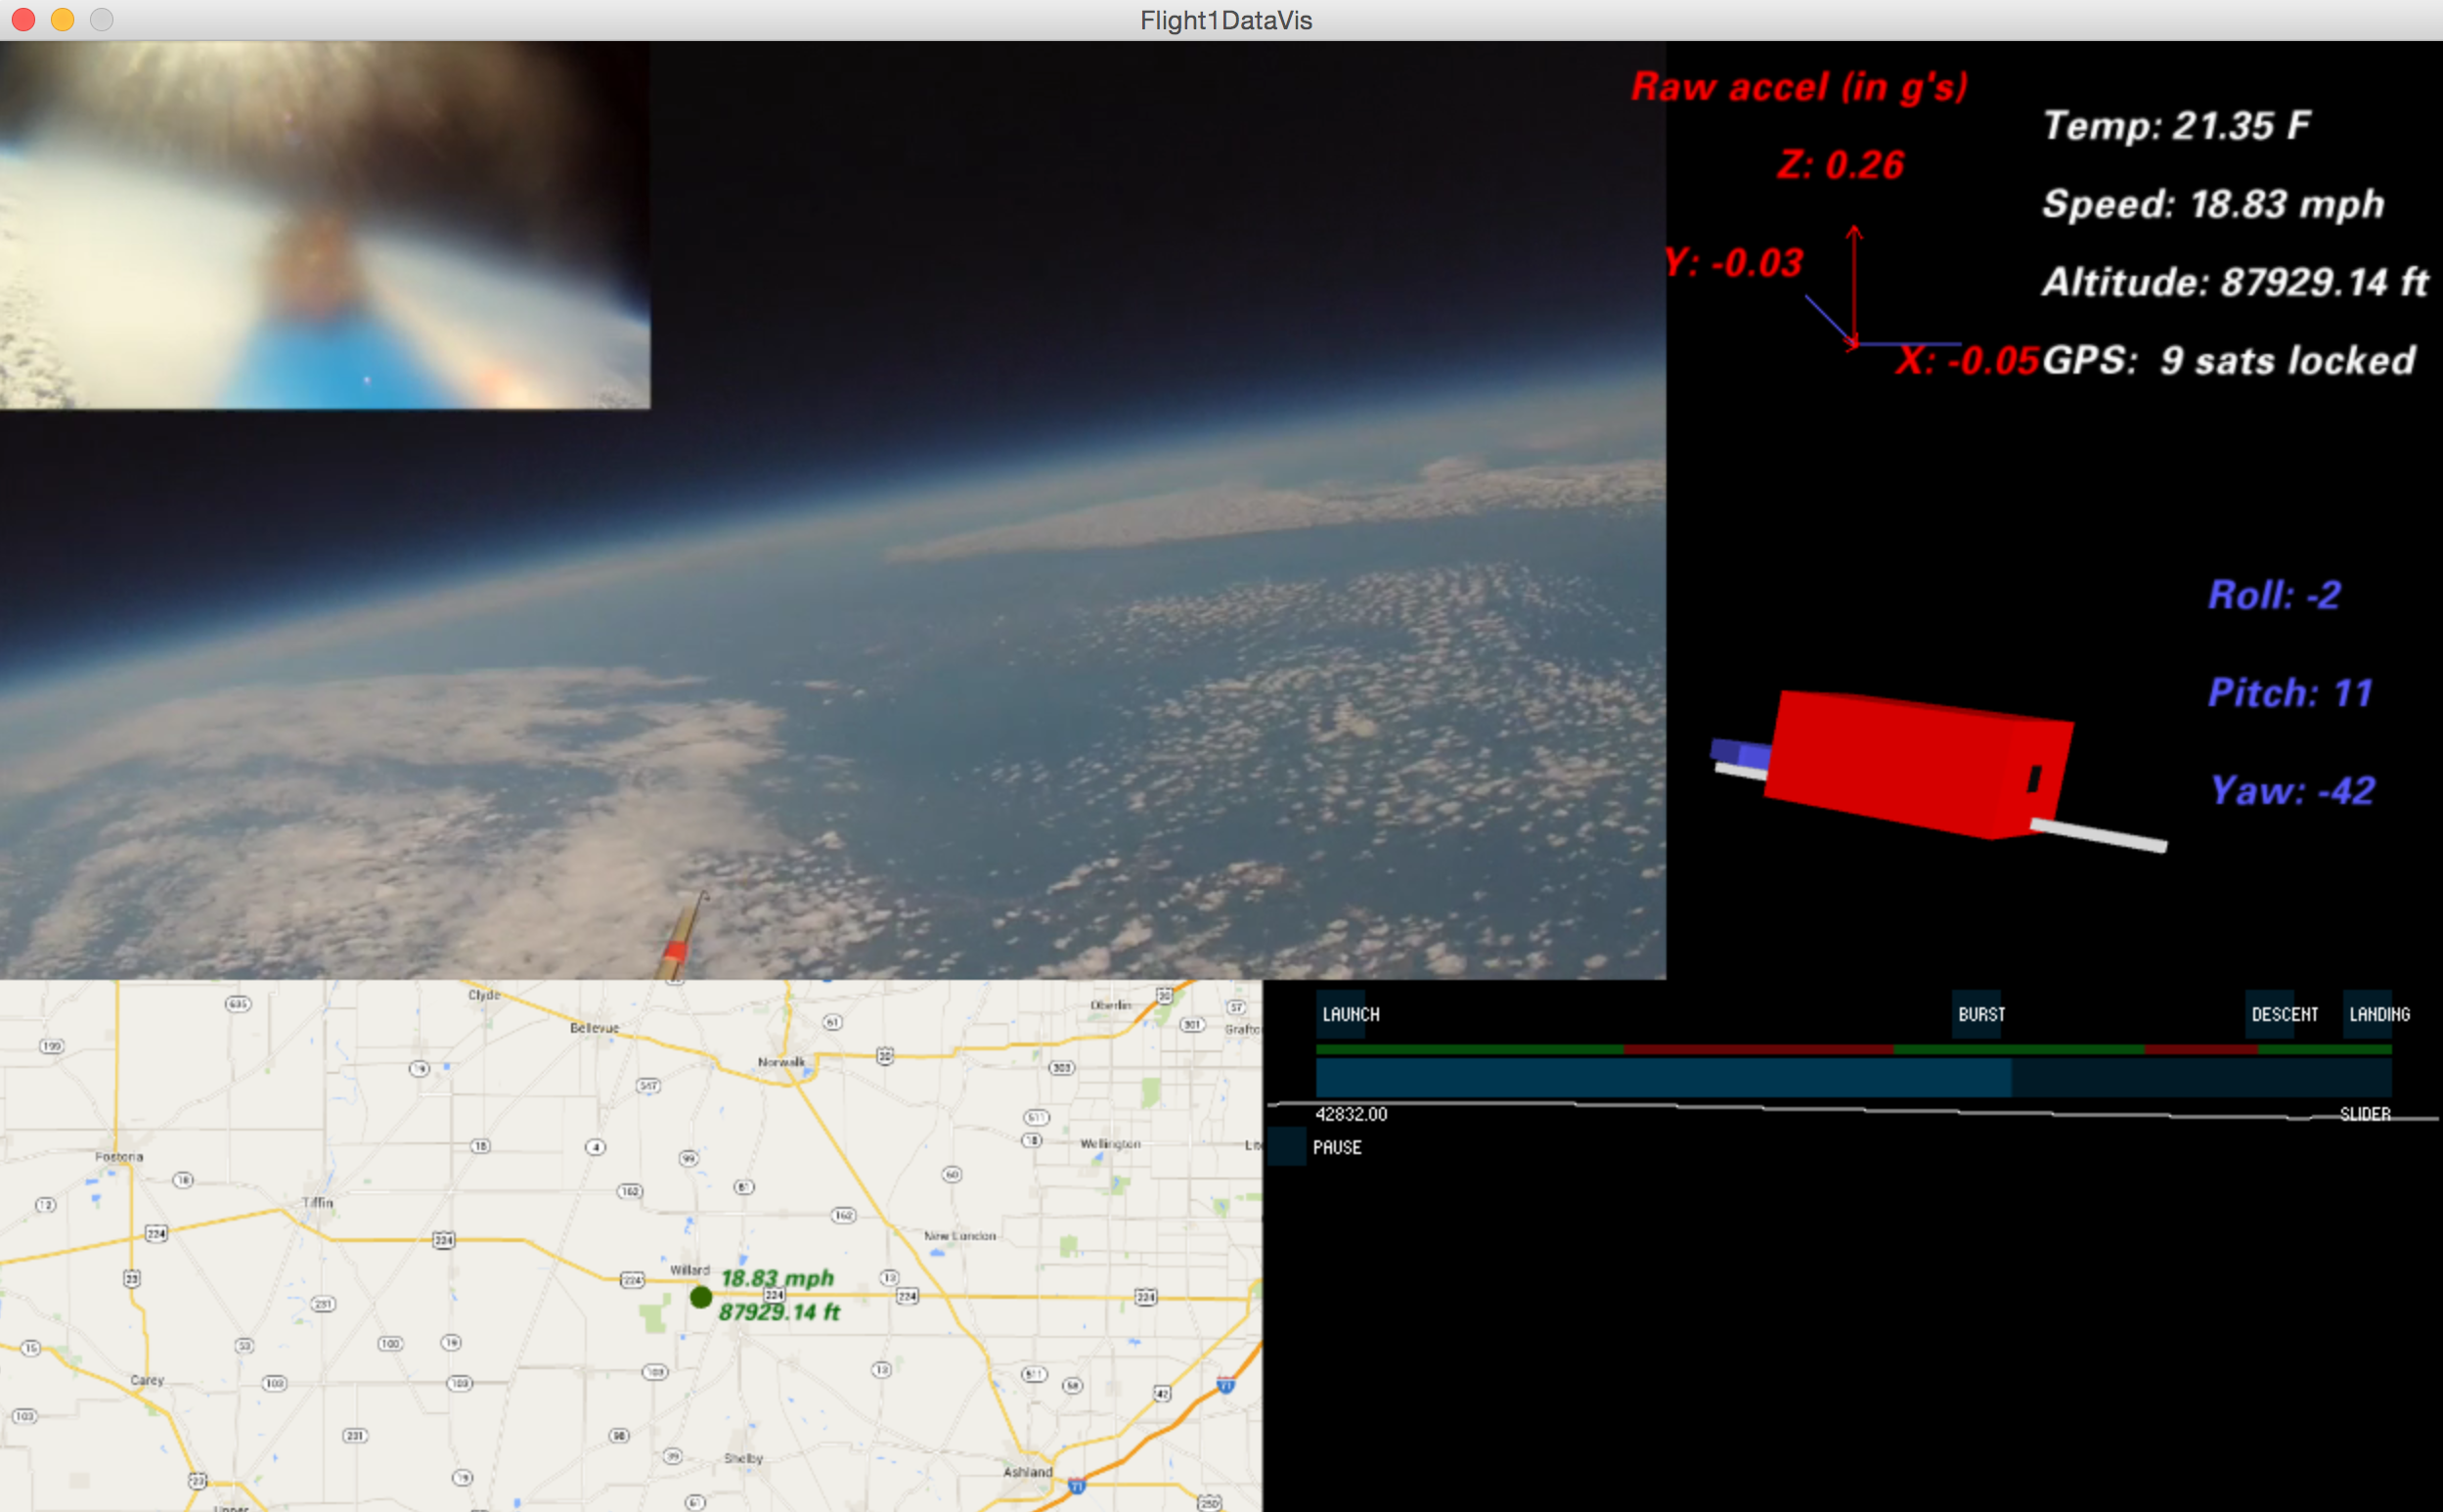
\includegraphics[width=1\textwidth]{images/space.png}
 \caption{Processing Visualization at 88kft}
\label{f:processing}
\end{figure}

This particular program displays the accelerations, temperature, speed,
altitude, and orientation in multiple contexts. There is a video component
showing a picture-and-picture view of both camera angles, accelerations plotted
as vectors, data shown as raw values, altitude shown both as a moving graph and
overlayed on a map with speed, and a 3D rendering of payload orientation.
The source-code for this visualization can be found in \cref{app:Github3}.
In order to properly sync the data with the video, all of the data was consolidated
into a single table, where data was reported in to a new row every 0.2 seconds.
The program embeds the video and syncs the framerate with rows of sensor data
from a CSV. At 30 frames per second, it reads a new row from the CSV file every
6 frames, updating the display. Playback controls are also provided, to allow
the user to skip to any segment of the video/database. This requires a video
file that starts and stops exactly with the beginning and endpoints of the data
file. This way jumping to the halway point, corresponds to exactly halfway down
the CSV file, and halfway through the video.

\subsection{Data Dissemination}

Two recommended services for online data dissemination include Github and
Google Fusion Tables.

\begin{figure}
\centering
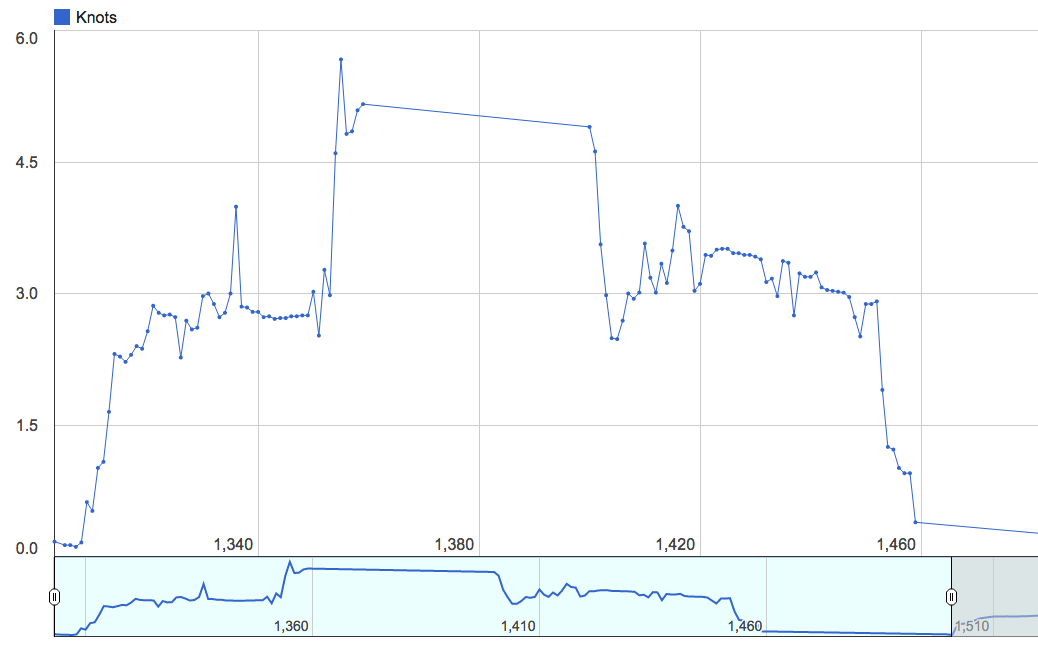
\includegraphics[width=1\textwidth]{images/speedPlot.png}
 \caption{Fusion Table Interactive Speed vs. Time Plot}
\label{f:plot}
\end{figure}

\begin{figure} [hbtp]
        \centering
        ~ %add desired spacing between images, e. g. ~, \quad, \qquad, \hfill etc.
          %(or a blank line to force the subfigure onto a new line)
        \begin{subfigure}[b]{0.45\textwidth}
                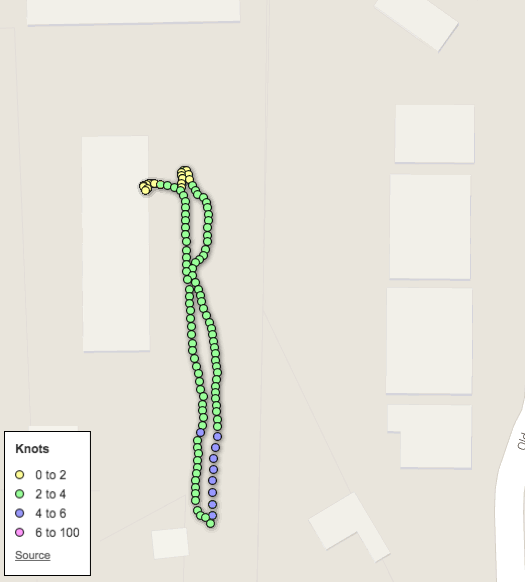
\includegraphics[width=\textwidth]{images/gps1.png}
                \caption{GPS with speed indicators}
                \label{fig:gps}
        \end{subfigure}
        ~ %add desired spacing between images, e. g. ~, \quad, \qquad, \hfill etc.
          %(or a blank line to force the subfigure onto a new line)
        \begin{subfigure}[b]{0.45\textwidth}
                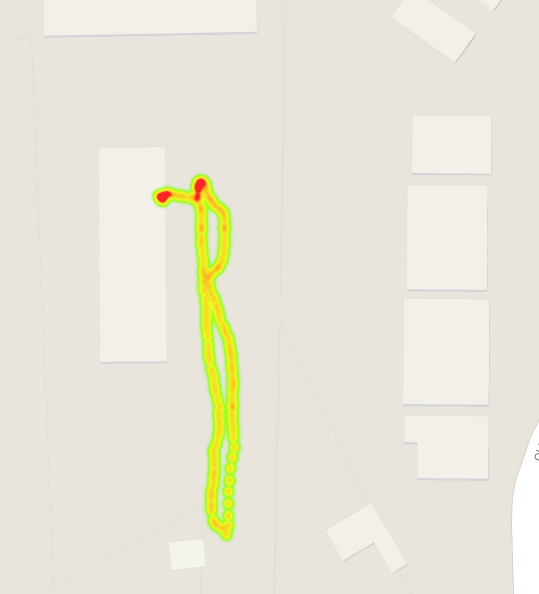
\includegraphics[width=\textwidth]{images/heatmap.png}
                \caption{GPS Heatmap}
                \label{fig:heatmap}
        \end{subfigure}
        \caption{Google Fusion Tables}
\end{figure}


\section{Final Remarks}

Ballon payloads offer extremely low-cost scientific platforms.
The advent of widely available inexepensive sensors, computers, and open-source
hardware/software have greatly reduced the barrier to entry for planetary
research.

The lightweight, inexpesnive sensor packages outlined in this paper can
scale to payloads of any size.
These systems were originally intended for passive monitoring systems,
however the final avionics system outlined could be used to control an
active descent system.

Balloons have made made a resurgance in both commercial and scientific applications.
Exiciting projects such as Google Loon are poised to play a large role in
extending internet connectivity to developing countries, proving that balloons
can have significant and impactful real-world applications. \cite{Loon}


\end{document}

